% The software this thesis built on and built, coloured by my role in each, with
% an arrow for every "depends on". The middle column holds what the CMB and the
% large-scale-structure sides share.
% Compile: see build.sh in this directory.
\documentclass[tikz,border=6pt]{standalone}
\usepackage{tikz}
\usepackage[T1]{fontenc}
\usetikzlibrary{arrows.meta,positioning,calc,backgrounds,fit}

\definecolor{ink}{HTML}{2E2E2E}
\definecolor{greytx}{HTML}{8A8A8A}
\definecolor{lead}{HTML}{C2560A}
\definecolor{coauth}{HTML}{521463}
\definecolor{contrib}{HTML}{3B6FB6}
\definecolor{cmbzone}{HTML}{FBF3EC}
\definecolor{lsszone}{HTML}{EEF3FA}

% #1 name  #2 position  #3 role colour  #4 label
\newcommand{\pkg}[4]{%
  \node[draw=#3,line width=1.3pt,fill=white,rounded corners=6pt,
        minimum width=2.75cm,minimum height=0.95cm,text=ink,
        font=\sffamily\small\bfseries]
       (#1) at #2 {#4};}

\begin{document}
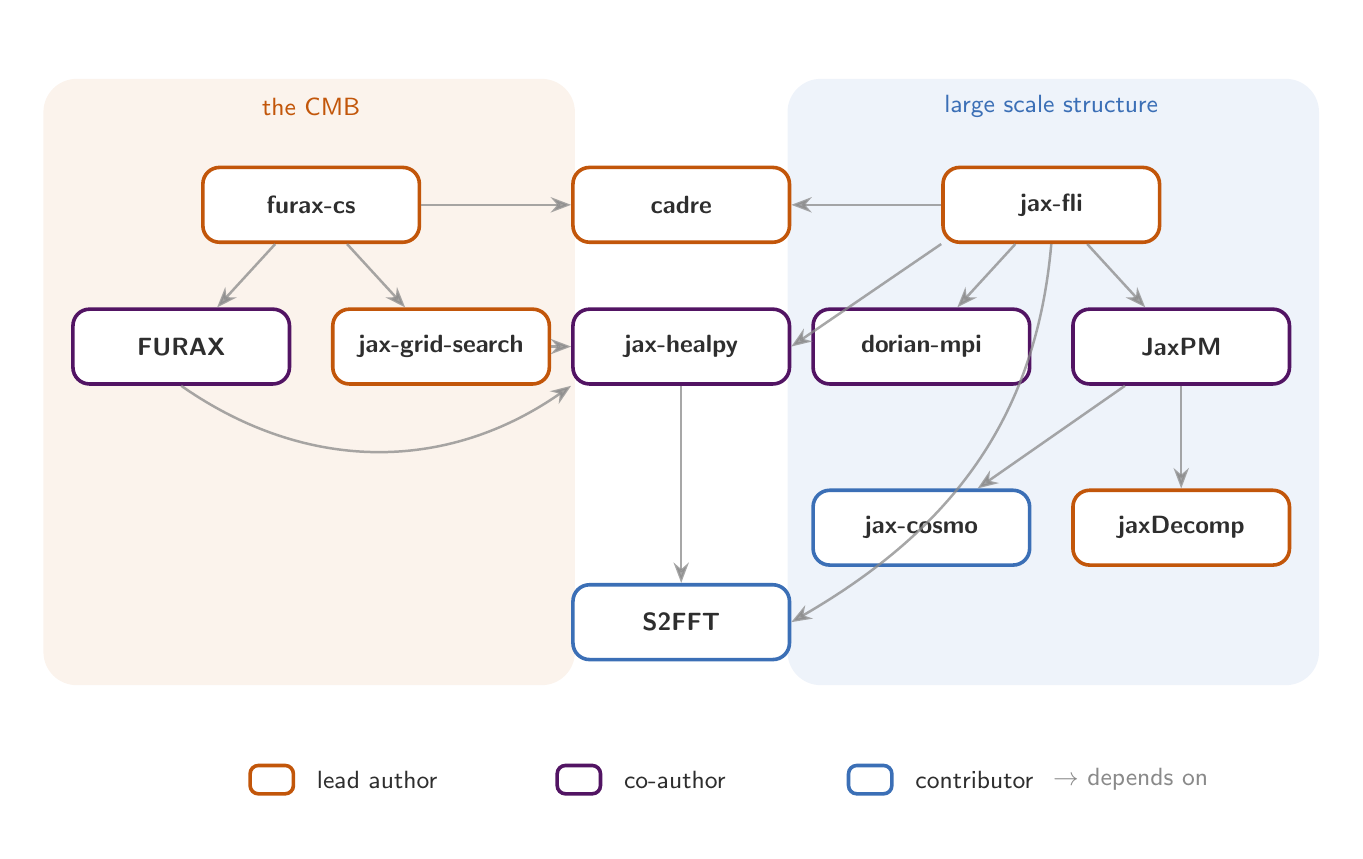
\begin{tikzpicture}
  \useasboundingbox (-8.3,-5.2) rectangle (8.3,5.0);

  % Two application areas behind the graph.
  \begin{scope}[on background layer]
    \fill[cmbzone,rounded corners=12pt] (-8.1,-3.35) rectangle (-1.35,4.35);
    \fill[lsszone,rounded corners=12pt] (1.35,-3.35) rectangle (8.1,4.35);
  \end{scope}
  \node[font=\sffamily\small,text=lead] at (-4.7,4.0) {the CMB};
  \node[font=\sffamily\small,text=contrib] at (4.7,4.0) {large scale structure};

  % CMB side
  \pkg{furaxcs}{(-4.7,2.75)}{lead}{furax-cs}
  \pkg{furax}{(-6.35,0.95)}{coauth}{FURAX}
  \pkg{gridsearch}{(-3.05,0.95)}{lead}{jax-grid-search}
  % LSS side
  \pkg{jaxfli}{(4.7,2.75)}{lead}{jax-fli}
  \pkg{jaxpm}{(6.35,0.95)}{coauth}{JaxPM}
  \pkg{dorian}{(3.05,0.95)}{coauth}{dorian-mpi}
  \pkg{jaxdecomp}{(6.35,-1.35)}{lead}{jaxDecomp}
  \pkg{jaxcosmo}{(3.05,-1.35)}{contrib}{jax-cosmo}
  % Shared
  \pkg{cadre}{(0,2.75)}{lead}{cadre}
  \pkg{healpy}{(0,0.95)}{coauth}{jax-healpy}
  \pkg{s2fft}{(0,-2.55)}{contrib}{S2FFT}

  \begin{scope}[-{Stealth[length=2.6mm]},greytx,line width=0.9pt,opacity=0.75]
    \draw (furaxcs) -- (furax);
    \draw (furaxcs) -- (gridsearch);
    \draw (furaxcs) -- (cadre);
    \draw (furax.south) to[out=-35,in=-145] (healpy.south west);
    \draw (gridsearch) -- (healpy);
    \draw (jaxfli) -- (jaxpm);
    \draw (jaxfli) -- (dorian);
    \draw (jaxfli) -- (cadre);
    \draw (jaxpm) -- (jaxdecomp);
    \draw (jaxpm) -- (jaxcosmo);
    \draw (jaxfli.south west) -- (healpy.east);
    \draw (healpy) -- (s2fft);
    \draw (jaxfli.south) to[out=-95,in=30] (s2fft.east);
  \end{scope}

  % Role legend
  \foreach \c/\t/\x in {lead/lead author/-5.2, coauth/co-author/-1.3,
                        contrib/contributor/2.4}{
    \node[draw=\c,line width=1.3pt,fill=white,rounded corners=3pt,
          minimum width=0.55cm,minimum height=0.36cm] at (\x,-4.55) {};
    \node[anchor=west,font=\sffamily\small,text=ink] at (\x+0.45,-4.55) {\t};}
  \node[anchor=west,font=\sffamily\small,text=greytx] at (4.6,-4.55)
       {$\rightarrow$ depends on};
\end{tikzpicture}
\end{document}
